\documentclass[a4paper, 11pt]{article}
\usepackage[utf8]{inputenc}
\usepackage[ngerman]{babel}
\usepackage{graphicx}
\usepackage{color}
\usepackage{tikz}
\usepackage{pgfplots}
\usepackage{amssymb}
\pagestyle{headings}


\begin{document}

\tableofcontents
\newpage

Das Travelling-Salesman Problem

\section{Einleitung}

\subsection{Geschichte}

Das Travelling-Salesman Problem ist ein Problem, das schon seit der Antike
besteht und die Menschen (und heute auch Maschinen) zum Nachdenken bringt:
Ein Bote/Handlungsreisender muss mehrere Städte besuchen und möchte den
kürzesten Weg finden, mit dem er jede Stadt exakt einmal in einer geschlossenen
Tour besuchen kann. \\

Wann das Problem ein erstes mal wissenschaftlich untersucht wurde ist unklar,
jedoch gab es im Jahre 1832 ein Handbuch für Handlungsreisende, das das Problem
zwar erwähnt aber nicht weiter behandelt.\\

Erstmals als Optimierungsproblem wurde das TSP im Jahre 1930 vom österreichischen
Mathematiker Karl Menger unter dem Titel \textit{Botenproblem}. Schon im
Vorhinein dieser Erwähnung gab es das \textit{Icosian Game} von William Rowan
Hamilton, der in einem Graphen Touren zwischen 20 Knoten finden wollte.\\

\subsection{Einsatzbereiche und Klassifikationen}

Heute hat das Travelling-Salesman Problem noch weitere, wichtige Einsatzbereiche
dazubekommen: So ergeben sich ähnliche Probleme bei der Genom-Sequenzierung, bei
der optimalen Plazierung von Bauteilen bei der Konzeption von Mikrochips, bei
der Tourenplanung von Logistikrobotern in großen Versandzentren (siehe Amazon)
oder bei der Tourplanung von Satelliten im Weltall um Sternenbilder zu erstellen.\\

Das Travelling-Salesman Problem selbst kann auch in mehreren Varianten (z.B.
bei einigen der vorher genannten Einsatzbereiche) auftreten. Eine mögliche
Variation ist das \textit{multiple TSP}, bei dem die Städte zusätzlich auf
mehrere Handlungsreisende aufgeteilt wird, wobei die Touren aller Reisenden
in der gleichen Stadt starten und enden müssen. Das multiple TSP kann noch
über das zusätzliche Kriterium, dass jeder Handlungsreisende mindestens zwei
Städte besuchen muss, zum schwierigeren \textit{multiple TSP with nonlazy
Salesmen} verschärft werden. Eine andere erwähnenswerte Variante ist das
\textit{Vehicle Routing Problem}, bei dem zusätzlich zu dem multiple TSP
Transportrestriktionen, wie z.B. Ladekapazitäten eines LKWs berücksichtigt werden
müssen. Weitere Variationen existieren, auf diese wird hier jedoch nicht näher
eingegangen.

\subsection{Schwierigkeiten}

Das Problem ist somit wichtig für viele Anwendungen, jedoch ist es bis heute
schwer, das Travelling-Salesman Problem exakt zu lösen: 1972 wurde die
\textit{NP-Vollständigkeit} des Hamiltonkreisproblems \footnote{
  Das Hamiltonkreisproblem beschreibt die Schwierigkeit einen
  geschlossenen Pfad in einem Graphen zu bestimmen, der jeden Knoten genau
  einmal enthält.
} festgestellt, aus dieser Feststellung ließ sich die NP-Vollständigkeit
des TSPs einfach herleiten. \\

In der folgenden Zeit bis heute wurden viele Anstrengungen unternommen, um das
TSP zu lösen oder zumindest näherungsweise zu bestimmen. Einige namhafte Algorithmen
zur näherungsweisen (auch möglicherweise optimalen) Lösung hierunter sind der
\textit{Kernighan-Lin-Algorithmus} oder auch \textit{Genetische Algorithmen}. Im
Folgenden soll aber genauer auf die Optimalen Verfahren wie auch teilweise auf deren
mathematische Grundlagen eingegangen werden.

\section{Analyse}

\subsection{Mathematische Betrachtung}

Im vorangehenden wurde oft der Begriff Städte für die Punkte verwendet, die
ein Handlungsreisender besuchen muss. Für die allgemeinere Definition wird
nun der Begriff \textit{Knoten} verwendet. \\

Ein TSP-Problem hat $N$ Knoten aus der Knotenmenge $V$. Zwischen allen Knoten
gibt es eine Verbindung, im Folgenden Kante genannt. Falls im ursprünglichen
Modell keine solche Kante existiert, so wird eine mit großer Länge eingefügt.
Zu jeder Kante zwischen einem Knoten $i$ und einem Knoten $j$ gibt es eine
Länge $c_{i,j} \geq 0$. \\

Um eine Tour zu beschreiben wird für jede Kante eine boolesche Variable $x_{i,j}$
eingeführt, wobei $i$ und $j$ jeweils unterschiedliche Knoten sind. Falls eine
Kante in einer Tour enthalten ist, so ist diese boolesche Variable $x = 1$,
ansonsten ist sie $0$. \\

Diese Bedingungen alleine genügen jedoch nicht: Falls man es nicht definieren
würde, wären somit Touren möglich, die durch einige Knotenpunkte mehrfach laufen
würden (siehe \ref{fig:multiple_connections_per_node}). Um solche Touren zu
vermeiden definiert man folgendes:

$$\sum_{j \in V \backslash i}x_{i,j} = 2$$

Die Summe aller Kanten, die in einen Knoten gehen, muss stets zwei sein (eine
eingehende und eine ausgehende Kante). \\

\begin{figure}[p]
    \centering
    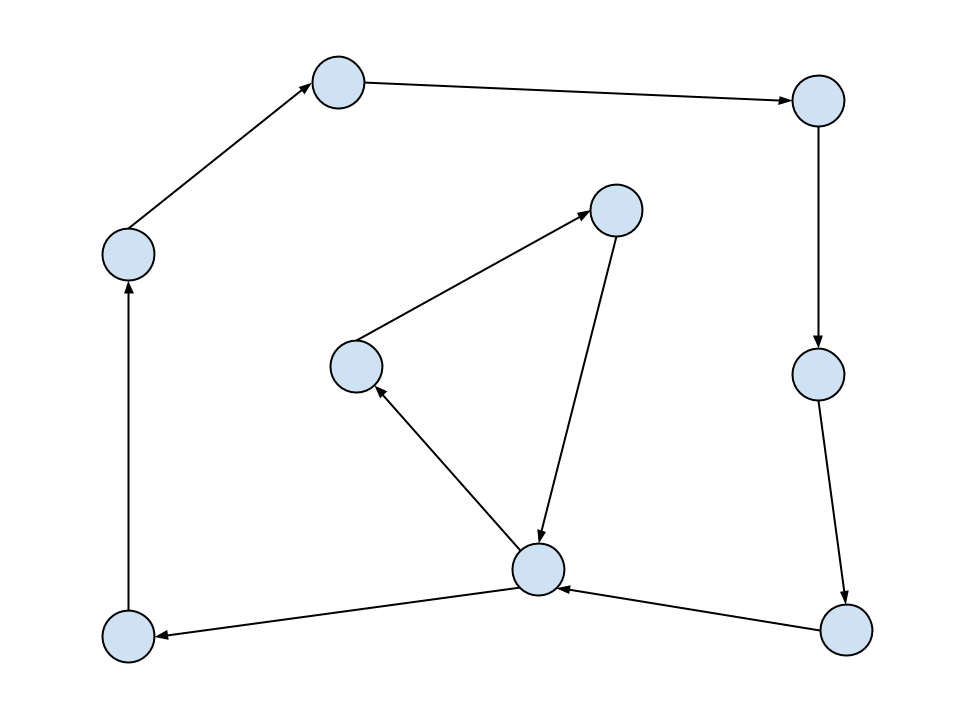
\includegraphics[width=0.8\textwidth]{invalid_tour.png}
    \caption{Drei Kanten zu einem Knoten}
    \label{fig:multiple_connections_per_node}
\end{figure}

Dennoch muss noch eine Bediungung definiert werden, damit eine Tour valide ist:
Momentan wäre eine Tour wie in \ref{fig:short_cycles} möglich, die sogenannte
\textit{Kurzkreiszyklen} enthält. Kurzkreiszyklen verletzen die Bedingung der
ein- und ausgehenden Kanten pro Knoten zwar nicht, jedoch entsteht so keine
zusammenhängende Tour. Um solche Touren zu verhindern definiert man deshalb
folgende Nebenbedingung:

$$\sum_{i \in S, j \notin S}x_{i,j} \geq 2$$

Hierbei werden zwei Mengen definiert: $S$ und $S^C$ (in der Formel mit
$j \notin S$). Eine Knotenmenge $V$ kann in $2^N$ verschiedene Mengen zerlegt
werden, weshalb man mit dieser Bedingung $2^N$ Nebenbedingungen hinzufügen
würde. Mathematisch gesehen ist diese Bedingung zwar zwingend notwendig, 
einige Programme zur Lösung eines TSPs fügen diese Bedingungen aber erst
dynamisch zur Laufzeit Schritt für Schritt hinzu. \\

Hat man nun eine valide Tour, so ist die Aufgabe, die Gesamtlänge der Tour
zu minimieren:

$$min\sum_{i \in V} \sum_{j \in V \backslash i} c_{i,j}x_{i,j}$$

\begin{figure}[p]
    \centering
    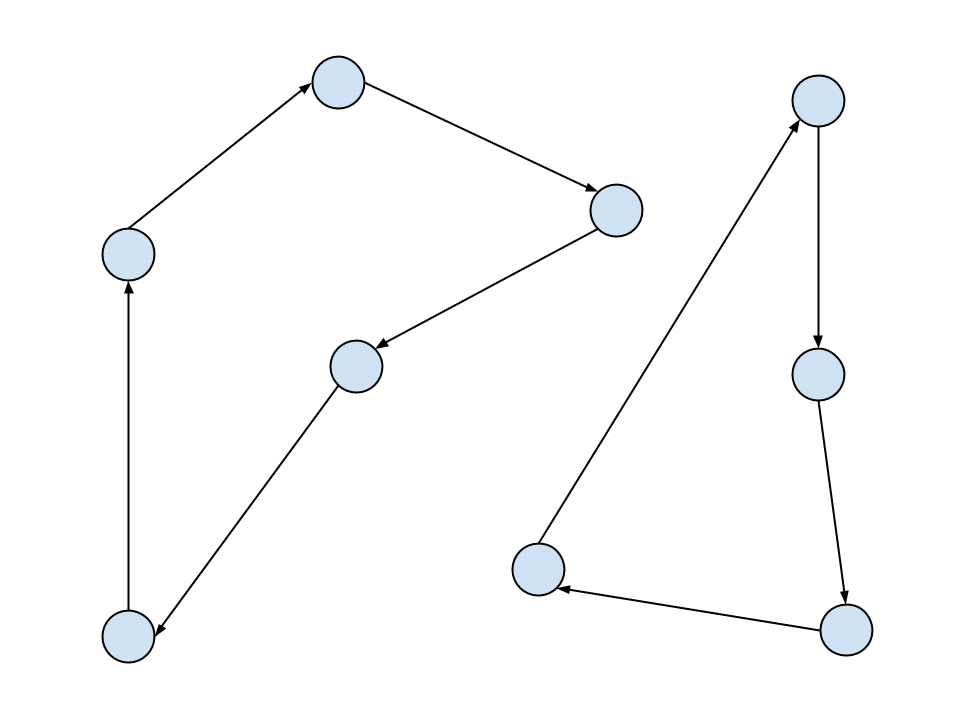
\includegraphics[width=0.8\textwidth]{kurzkreiszyklen.png}
    \caption{Kurzkreiszyklen innerhalb einer Tour}
    \label{fig:short_cycles}
\end{figure}

\subsection{Klassifikationen}

Wie schon zuvor gesehen, kann ein TSP in verschiedenen Variationen auftreten.
Es existieren deshalb einige Klassifikationen für TSPs:

\begin{itemize}
  \item Symmetrische TSPs sind TSPs bei denen der Hin- und der Rückweg stets
  gleich lang ist. Mathematisch wird dies beschrieben durch
  $c_{i,j} = c_{j,i}$. Ein TSP, das symmetrisch ist, ist beispielsweise das
  \textit{Euklidische TSP}, bei dem Knoten Punkte im zweidimensionalen Raum
  sind.

  \item Das ``Gegenstück'' zu symmetrischen TSPs sind asymmetrische TSPs.
  Bei diesen TSPs muss die Bedingung, dass Hin- und Rückweg gleich lange
  sind, nicht immer erfüllt sein. Ein asymmetrisches TSP ist z.B. im Alltag
  gegeben, wenn man beim Hinweg über Einbahnstraßen relativ direkt von A
  nach B kommt, aber man beim Rückweg diese Einbahnstraßen nicht nutzen kann.

  \item Metrische TSPs erfüllen die \textit{Dreiecksungleichung}. Die
  Dreiecksungleichung lautet $c_{i,j} \leq c_{i,k} + c{k, }$ und beschreibt,
  dass eine Strecke von einem Punkt $i$ zum Punkt $j$ immer kürzer sein
  muss als die Strecke über einen dritten Punkt $k$. Ein nicht-metrisches
  TSP ist gegeben, wenn beispielsweise Umrüstzeiten berücksichtigt werden
  müssen.
\end{itemize}

\subsection{Komplexität}

Die Anzahl der Touren bei einem asymmetrischen TSP sind $(N - 1)!$ (
Entscheidungsbaum pro Kante). Bei einem symmetrischen TSP gibt es
$\frac{N - 1}{2}$ Touren (da der Hin- und Rückweg zwischen zwei Kanten
derselbe ist halbiert sich die Anzahl der möglichen Touren).\\

Falls man sich einmal nicht in einem euklidischen TSP befindet muss man
auch die Kantenlängen errechnen. Würde man dies für ein Problem mit
$N = 1000$ (1000 Städte) tun, so hätte man erst einmal 1.000.000 mögliche
Verbindungen. Diese Für jede dieser Verbindungen müsste man, z.B. bei einem
Straßennetz, einen Dijkstra-Durchlauf starten. Ein Dikjstra-Durchlauf benötigt
bei beispielhaften Bedingungen ca. 10s, daraus resultiert eine Laufzeit von $\approx$
116 Tagen. In der Praxis verwendet man deshalb häufig die Luftlinie zwischen
zwei Städten multipliziert mit $1.3$ als Approximation (für die meisten
Umgebungen hinreichend genau).

\section{Exakte Lösungen}

\subsection{Permutation}

Das TSP kann gelöst werden, indem man durch alle möglichen Touren permutiert.
Für kleine $N$ ist dies noch möglich, jedoch die Anzahl an Touren wächst
drastisch mit größeren Knotenanzahlen (siehe \ref{fig:faculty_graph}). Ein
effizienteres Verfahren muss also bestimmt werden.

\begin{figure}
  \centering
  \begin{tikzpicture}[scale=0.6]
    \begin{axis}[
        symbolic x coords={3, 4, 5, 6, 7, 8},
        xtick=data
      ]
        \addplot[ybar,fill=blue] coordinates {
            (3, 1)
            (4, 3)
            (5, 12)
            (6, 60)
            (7, 360)
            (8, 2520)
        };
    \end{axis}
  \end{tikzpicture}
  \label{fig:faculty_graph}
  \caption{Anzahl Touren in Abhängigkeit $n$ bei symmetrischem TSP}
\end{figure}

\subsection{Lineare Programmierung}

Ein Verfahren, das bei erster Betrachtung nicht als ein Verfahren zur Lösung
des TSPs anmutet ist die Lineare Programmierung. Bei der Linearen Programmierung
werden Probleme mit einer Zielfunktion und mehreren Nebenbedingungen,
sogenannten \textit{Constraints} gelöst.

\subsubsection{Mathematische Beschreibung}
Bei einem linearen Programm ist eine Matrix $A \in \mathbb{R}^{m,n}$ sowie
zwei Vektoren $b \in \mathbb{R}^m$ und $c \in \mathbb{R}^n$ gegeben. Der
Vektor $b$ formuliert die Constraintwerte, $c$ die Zielfunktion und $A$ die
einzelnen Constraintgleichungen. Ziel ist es, einen
zulässigen Vektor $x$ zu finden, der das Standardskalarprodukt
$c^Tx = c_1x_1 + \ldots + c_nx_n$ maximiert. Falls man minimieren statts
maximieren will, so multipliziert man $c$ mit $-1$. 

\end{document}